\documentclass[a4paper,11pt]{article}
\usepackage{amssymb}
\usepackage{booktabs}
\usepackage{geometry}
\usepackage{color}
\usepackage{hyperref}
\usepackage{listings}
\usepackage{graphicx}
\usepackage{float}
\usepackage{caption}
\usepackage{subcaption}
\usepackage[T1]{fontenc}
\usepackage{algo}

\geometry{
	includeheadfoot,
	margin=2.54cm
}

\setlength\parindent{24pt}

\title{
	2IL76 Algorithms for Geographic Data Set 4 \\
}
\author{
	Bram Kohl - b.j.e.kohl@student.tue.nl - 0746107
}
\date{\today}

\begin{document}
	\maketitle
	
\section*{Exercise 1}
We have to prove that using unit-square labels, the 4-slider model can sometimes label 1.5 times as many points as any fixed position model. So for any fixed position model there is an instance of points of which the 4-slider model can label 1.5 times as many points as the fixed position model.\\

The fixed position model can have any number of admissable positions on the boundary, so in order to prove this we use the fact that there is a position on the bottom of the boundary of the unit square which is not one of the fixed position model positions. As we will see later, we need a point on the top of that boundary, across from the other point as well. There cannot be an infinite number of admissable positions on the boundary of the unit square in the fixed position model (that would be a slider model). So there have to be two points across from eachother of which neither are in the fixed position model, otherwise we would still need an infinite number of points on the boundary.\\
To make this more clear, let's say these positions are the ones shown in figure \ref{fig:notinmodel}.\\


\begin{figure}[H]
	\centering
	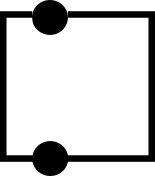
\includegraphics[scale=0.3]{4-1.png}
	\caption{The shown positions are exactly across from eachother (same x) and are not in this fixed position model}
	\label{fig:notinmodel}
\end{figure}

Now we show that there is an instance of points which need precisely these position to be able to place a label on all points, which causes it to miss these points. The instance we choose is created by taking the unit squares for which we cannot pick a point, and placing them as seen in figure \ref{fig:pointplacement}. Then we add two points at the sides of each unit square, which can be seen in figure \ref{fig:pointplacement} as well. This results in the pointset in figure \ref{fig:pointset}

\begin{figure}[H]
	\centering
	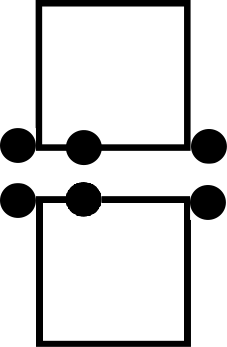
\includegraphics[scale=0.3]{4-3.png}
	\caption{This figure shows how the remaining points are chosen}
	\label{fig:pointplacement}
\end{figure}

\begin{figure}[H]
	\centering
	
\includegraphics[scale=0.3]{4-2.png}
	\caption{The resulting pointset}
	\label{fig:pointset}
\end{figure}

Due to the way we chose the points (as described above), the leftmost and rightmost points are exactly one unit-square apart. So the 4-slider model can label all 6 points in the way shown in figure \ref{fig:labelplacement}. Note that this is not an exact representation of the label placement, as due to the thickness of the points there is still some space between the labels that are next to eacother.\\

\begin{figure}[H]
	\centering
	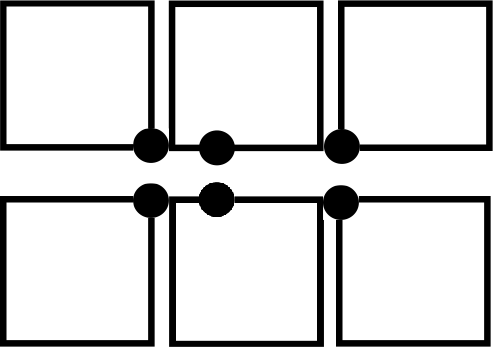
\includegraphics[scale=0.3]{4-4.png}
	\caption{Labeling for the pointset in figure \ref{fig:pointset} with the 4-slider model}
	\label{fig:labelplacement}
\end{figure}

So given the fixed position model with these admissable positions missing we can create a pointset, using these missing positions, which has 6 points of which only 4 can be labeled by the fixed position model, because if we move the middle labels from figure \ref{fig:labelplacement} a little to the right or left, we immediately get a conflict with the label next to it. As the non-admissable positions are exactly across from eachother, it is not possible to place 5 labels either (which could otherwise be done by putting the top middle label underneath the point and deleting the bottom label, or the other way around).\\

Thus we found a pointset for which the 4-slider model can label $\frac{6}{4} = 1.5$ times as many points as any fixed position model.


\section*{Exercise 2}
\end{document} 